\chapter{Demonstration of Utility}\label{ch:demonstration}
This chapter demonstrates the practical utility of the reliability model introduced in \chref{ch:reliable-sots} by implementing its concepts within a concrete system architecture. The Level~4 adaptive reliability mechanisms are implemented in a proof-of-concept middleware supporting a CEP-based SoTS. In this running example, constituents produce observations that are converted into events and analysed by a CEP service. Executable lifecycle statecharts regulate how observations contribute to system-level reasoning and when compensation mechanisms reconstruct missing observations during constituent degradation.

The chapter first presents the system architecture used to realize the reliability model (\secref{sec:architecture}). It then describes the implementation of the CEP-based middleware (\secref{sec:implementation}) and explains how executable lifecycle statecharts enforce participation constraints, including compensation and estimation under restricted roles (\secref{sec:statechart-behaviour}). Finally, the chapter introduces the experimental setup used to evaluate the impact of lifecycle control and compensation on system reliability (\secref{sec:evaluation}).


\section{System Architecture}\label{sec:architecture}
This section presents the architecture used to realize a Level~4 reliable SoTS within the CEP-based running example introduced in \chref{ch:introduction}. In this setting, constituent observations are transformed into events and processed to detect system-level behaviour, while lifecycle statecharts regulate how constituents participate and contribute.

\subsection{Architectural Realization of Level~4 SoTS Adaptive Reliability}
The Level~4 adaptive reliability model (see \secref{sec:lv4}) introduces requirements for regulating participation and limiting the influence of degraded constituents. These motivate architectural mechanisms for state-aware event production, compensation, and controlled contributions. At the core, executable lifecycle statecharts controls when constituents contribute and how their behaviour is constrained. To realize this within the CEP infrastructure, a set of architectural components is introduced, derived directly from Level~4 to support these behaviours.

The resulting architecture is structured around the following key mechanisms:

\begin{itemize}
    \item \textbf{State-aware contribution control:} The \textit{Event Source} component interacts with lifecycle statecharts to ensure that event emission is enabled, suppressed, or modified based on the constituent's current belonging state and participation role.
    
    \item \textbf{Compensation-enabled participation:} The \textit{Event Compensator} component, including the \textit{Reconstructor} and \textit{Predictor}, supports continued participation during periods of instability. Constituents in \textit{Restricted Role} contribute through estimated observations when direct outputs are unreliable.

    \item \textbf{Uncertainty-bounded contribution:} Compensation outputs include confidence measures that are evaluated against thresholds. When uncertainty exceeds acceptable limits, the \textit{Lifecycle Manager} component enforces transitions that restrict or terminate participation.

    \item \textbf{Separation of observation and system-level reasoning:} The \textit{Event Stream} and \textit{Event Processor} components isolate event production from higher-level behaviour detection, ensuring that only validated or compensated observations influence system-level reasoning.
\end{itemize}

\subsection{Component Model of Architecture}

\figref{fig:component-model} illustrates the architectural components derived from the Level~4 adaptive reliability model. At the centre of the architecture, the \textbf{Lifecycle Manager}, implemented using executable statecharts, governs constituent participation by enforcing role transitions and contribution constraints. \textbf{Event Sources} generate events from observations in accordance with lifecycle state. These events are distributed via the \textbf{Event Stream} and analysed by the \textbf{Event Processor} to detect higher-level system behaviour. When disturbances affect event availability or reliability, the \textbf{Event Compensator} reconstructs observations to allow constituents to remain active under constrained conditions.

\begin{figure}[htp]
\centering
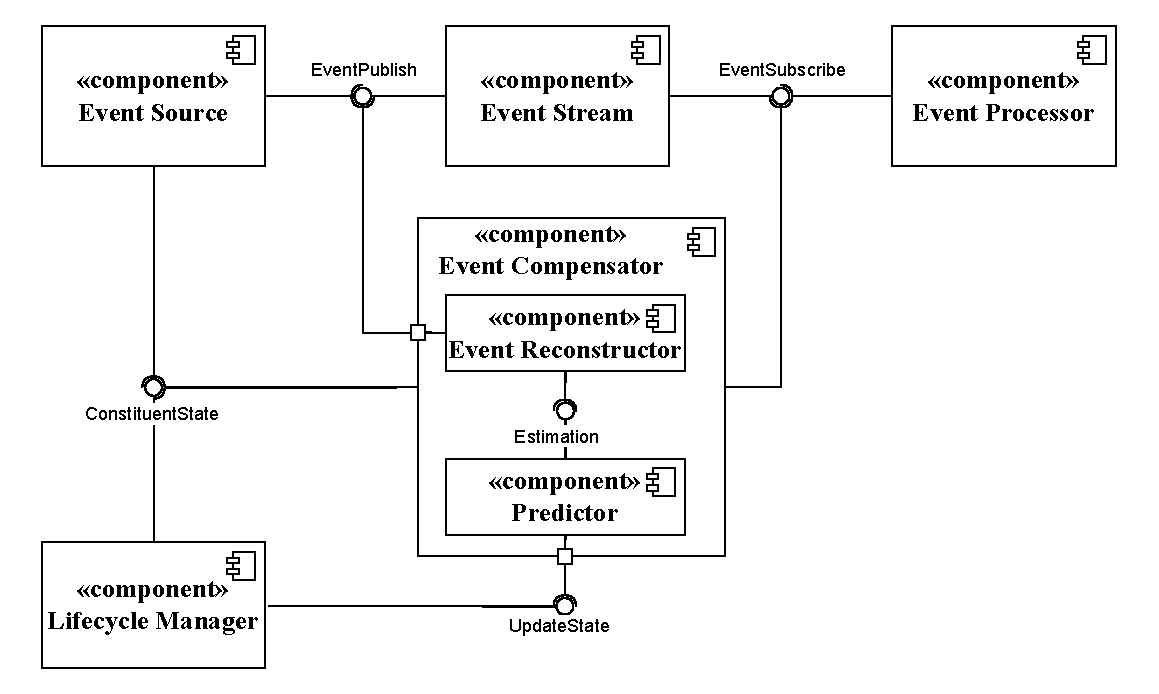
\includegraphics[width=0.65\textwidth]{figures/Architecture/High Level Component Diagram.drawio.pdf}
\caption{Component model of the demonstrated architecture}
\label{fig:component-model}
\end{figure}

The primary architectural components are:

\begin{itemize}

\item \textbf{Lifecycle Manager} maintains the lifecycle state of each constituent using executable statecharts and enforces adaptive participation constraints based on health conditions and uncertainty thresholds.

\item \textbf{Event Source} converts observations into events and publishes them to the event stream in accordance with lifecycle state and participation role, enabling state-aware control over contribution.

\item \textbf{Event Stream} distributes events between producers and consumers using a publish-subscribe model, decoupling event production from system-level processing.

\item \textbf{Event Processor} consumes events and detects higher-level system behaviours through event pattern detection, operating only on validated or compensated inputs.

\item \textbf{Event Compensator} monitors the event stream and supports continued participation during periods of instability by reconstructing missing or unreliable observations. It evaluates the confidence of reconstructed outputs and signals when uncertainty exceeds acceptable bounds, enabling the Lifecycle Manager to restrict or terminate participation.

\begin{itemize}
\item \textbf{Event Reconstructor}, which generates and publishes reconstructed events to the stream.
\item \textbf{Predictor}, which estimates expected measurements used during reconstruction.
\end{itemize}

\end{itemize}

\section{System Implementation}\label{sec:implementation}
The architecture is implemented as an event-driven middleware with Python-based coordination services and a Java-based CEP engine. The Python layer manages lifecycle state and event generation via a \textit{lifecycle manager} implemented using Itemis CREATE statecharts. Events are transmitted through a ZeroMQ-based \textit{event stream} and processed by an \textit{event processor} built with Esper CEP Engine. An \textit{event compensator} monitors the stream and reconstructs events when needed using a Kalman filter-based \textit{predictor}.


\subsection{UML Model of Implementation}
\begin{figure}[htp]
\centering
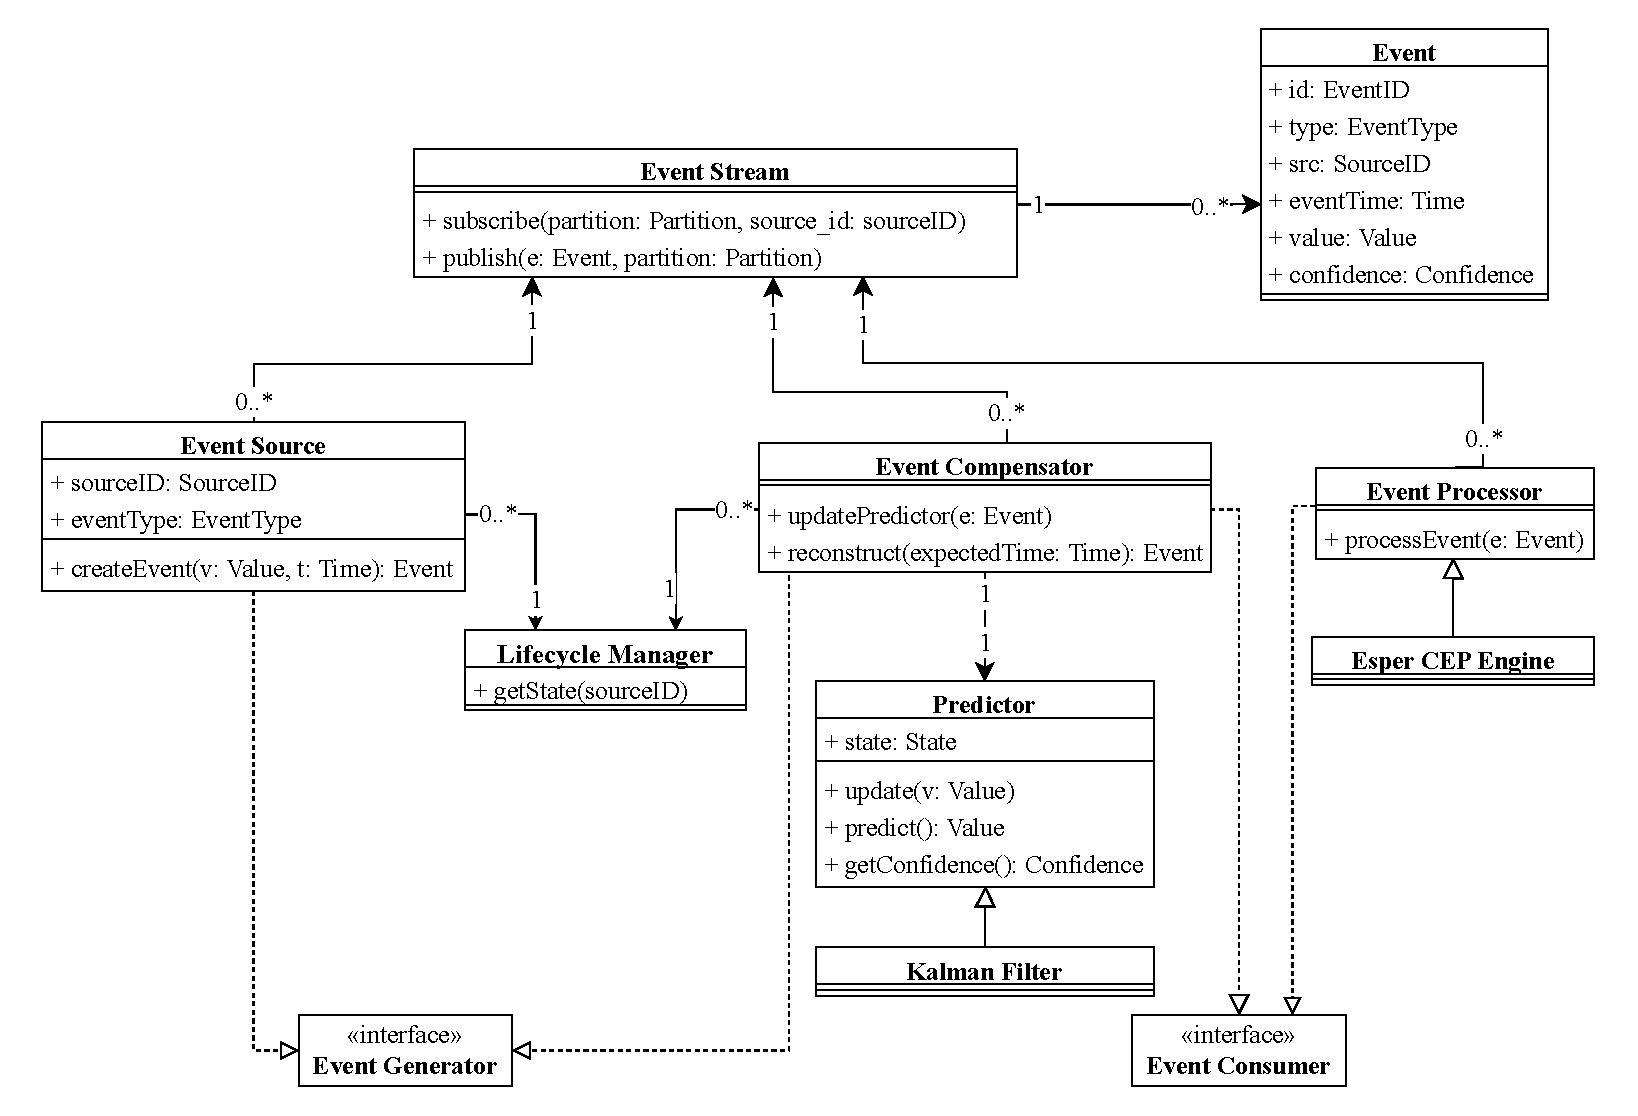
\includegraphics[width=0.9\textwidth]{figures/Architecture/UML Model.drawio.pdf}
\caption{UML model of architecture}
\label{fig:uml-model}
\end{figure}
\figref{fig:uml-model} presents the runtime structure of the system using a UML component model. \textit{Event Generator} and \textit{Event Consumer} define abstract roles for components that produce and consume events, respectively. The \textit{event source} realizes the \textit{Event Generator} interface, while both the \textit{event processor} and \textit{event compensator} act as \textit{Event Consumers}. The \textit{event stream} provides a transport mechanism between generators and consumers, with publish-subscribe interactions indicated through associations. The \textit{event compensator} maintains an internal \textit{predictor}, implemented as a Kalman filter, to support reconstruction. The \textit{lifecycle manager} is queried by other components to obtain the current participation state.

\subsection{Enforcing the SoTS Reliability Model with Executable Statecharts}\label{sec:statechart-behaviour}
The reliability model introduced in \secref{sec:reliability-levels} defines lifecycle constraints governing how constituents participate and contribute in a SoTS. In this implementation, these constraints are enforced through executable lifecycle statecharts associated with each constituent, which maintain belonging and health states. Event publishing and compensation behaviours are determined by the constituent's current state, allowing the lifecycle model to directly govern runtime behaviour.

\subsubsection{Executable Statecharts with Itemis CREATE}\label{sec:itemis-create}
\begin{figure}[htp]
\centering
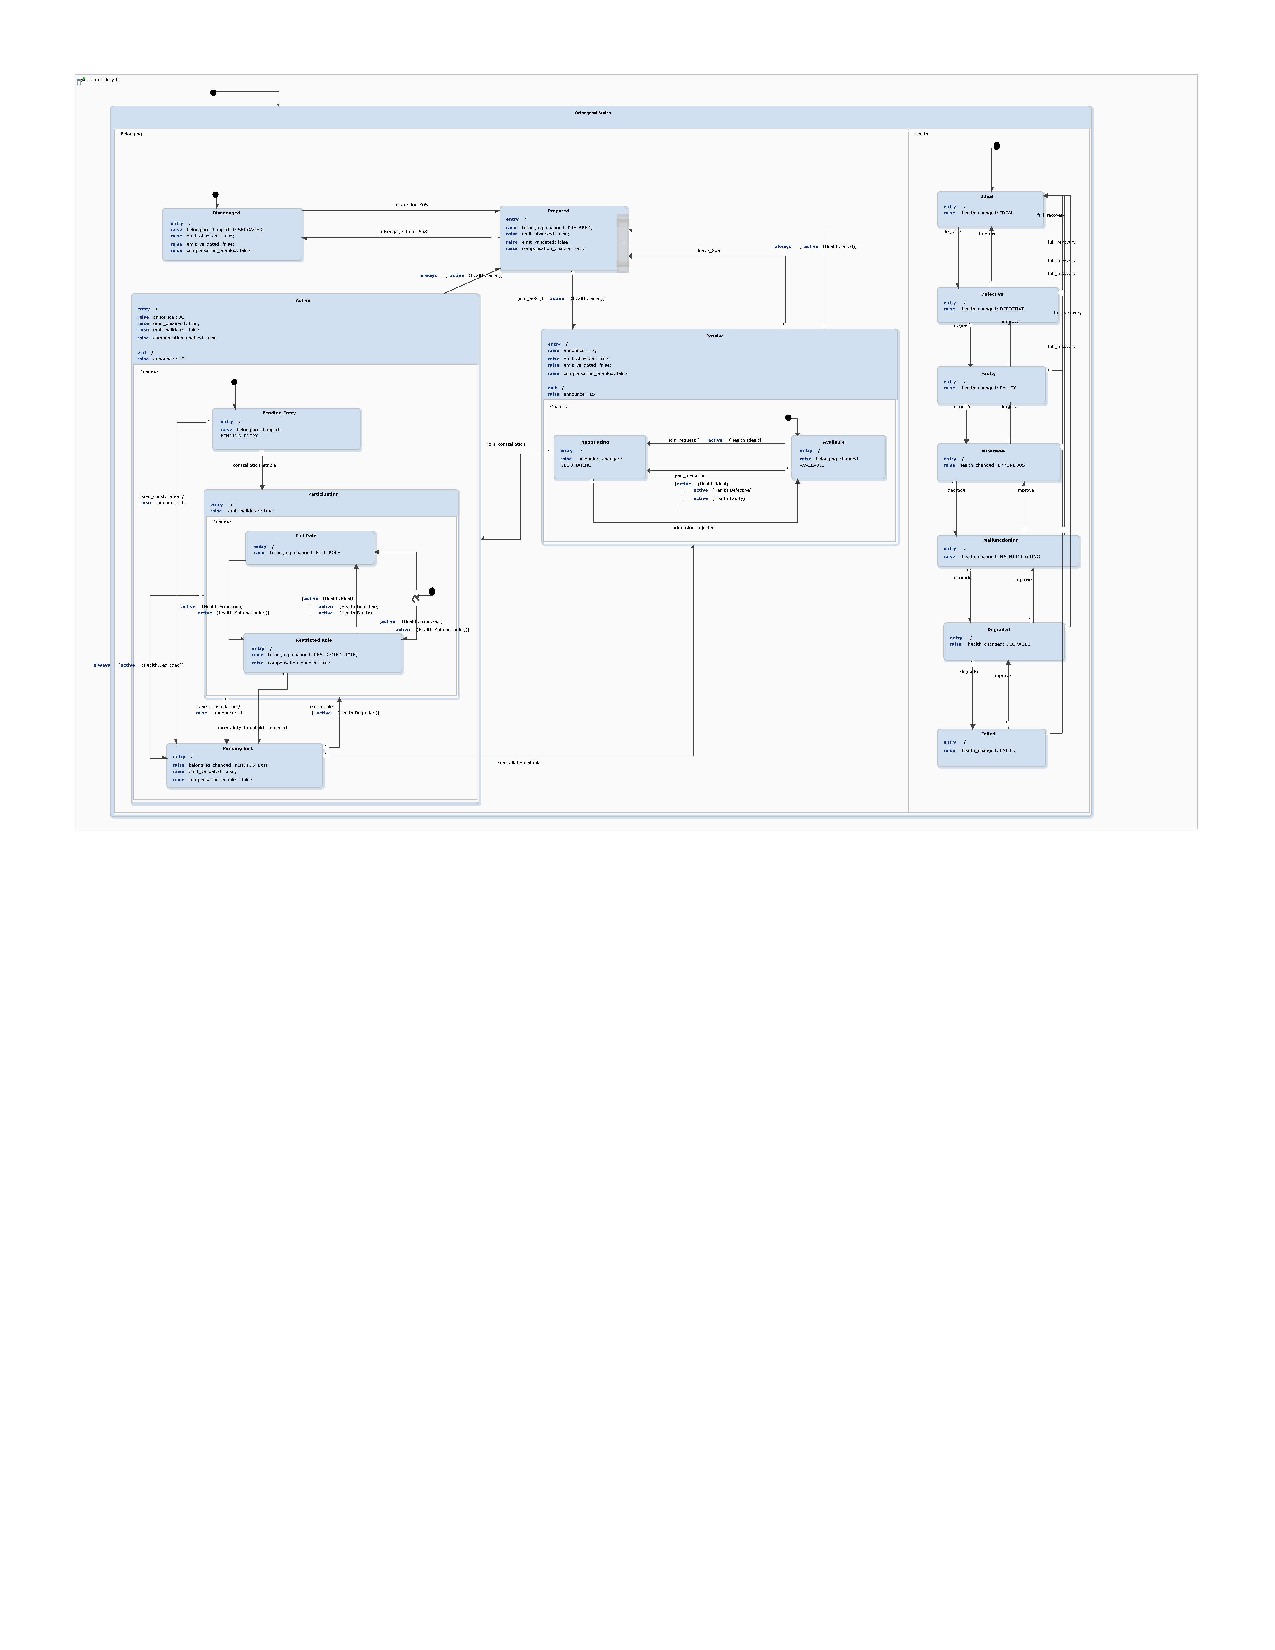
\includegraphics[
        width=0.85\linewidth,
        trim=2cm 14cm 2cm 2cm,
        clip
    ]{figures/Architecture/itemis.pdf}
\caption{Statechart Model in itemis CREATE}
\label{fig:itemis-diagram}
\end{figure}
Lifecycle statecharts are implemented using Itemis CREATE\footnote{{itemis CREATE is a statechart modelling and code generation environment developed by itemis AG. See: \url{https://www.itemis.com/en/products/itemis-create}.}}, which provides a modelling environment for defining state machines and generating executable code. The Python code generator compiles lifecycle models into executable controllers integrated into the runtime system, where each constituent is associated with a statechart instance exposing lifecycle states, transitions, and events through a runtime interface.

Itemis CREATE also generates observable streams for statechart events, enabling a reactive execution model. System components subscribe to these observables and update their behaviour in response to emitted signals (e.g., enabling or disabling event emission or compensation). This establishes reactive coupling between lifecycle models and system behaviour, ensuring that coordination policies defined in the statechart are enforced automatically at runtime.

\subsubsection{Statechart-Controlled Runtime Behaviour}
The system enforces the Level~4 adaptive reliability model (\secref{sec:lv4}) within the CEP-based SoTS. Lifecycle state governs participation, and thus contributions, as health evolves. Both event sources and the compensation service consult the controller to determine when emission, updates, and reconstruction are permitted. Table~\ref{tab:state-behaviour} summarizes the behaviours associated with each lifecycle state.

\begin{table}[htp]
\small
\centering
\caption{Lifecycle state effects on events, compensation, and prediction}
\label{tab:state-behaviour}
\begin{tabular}{l c c c}
\toprule
\textbf{Lifecycle State} 
& \makecell{\textbf{Contributes} \\ \textbf{Events}} 
& \makecell{\textbf{Uses} \\ \textbf{Compensation}} 
& \makecell{\textbf{Updates} \\ \textbf{Predictor}} \\
\midrule


Disengaged &  &  &  \\
Prepared &  &  &  \\

\midrule
Passive (Negotiating) &  &  & $\checkmark$ \\
Passive (Available) &  &  & $\checkmark$ \\

\midrule
Active (Pending Entry) &  &  & $\checkmark$ \\
Active (Full Role) & $\checkmark$ &  & $\checkmark$ \\
Active (Restricted Role) & $\checkmark$ & $\checkmark$ & $\checkmark$ \\
Active (Pending Exit) &  &  & $\checkmark$ \\

\bottomrule
\end{tabular}
\end{table}

\paragraph{Event Contribution and Consumption}
Belonging in the SoTS is tied to providing capability, represented in the CEP-based running example by supplying events for processing. In \textit{Active} states, constituents emit events to the stream for system-level processing. In \textit{Passive} states, events are used only for internal processing. In \textit{Prepared} and \textit{Disengaged} states, constituents do not contribute to the event stream.

\paragraph{Event Reconstruction}
When health degrades and a constituent transitions to the \textit{Restricted Role}, observations may become incomplete or unavailable. In this case, the compensation service reconstructs missing events to maintain a consistent event stream, allowing continued participation while limiting the effects of degraded sensing or communication.

\paragraph{Estimator Updates}
The state estimator updates whenever observations are available. Updates therefore occur across \textit{Passive} and \textit{Active} states, maintaining an internal estimate of system behaviour even when participation not actively participating.


\subsection{Compensation under Restricted Roles}\label{sec:demo-compensation}
The \textit{Restricted Role} introduced in Level~4 allows degraded constituents to continue participating while limiting their influence on system-level reasoning. Within this role, compensation is tightly integrated with lifecycle statecharts: reconstructed observations are accompanied by a confidence measure that directly controls behavioural transitions. As long as confidence remains within acceptable bounds, the constituent may continue operating in a restricted capacity; otherwise, the statecharts enforce withdrawal to prevent unreliable contributions from affecting the system.

\paragraph{State Estimation for Compensation}
In the CEP-based SoTS, disturbances caused by unavailable observations are addressed through an estimation-based compensation service \cite{hanmer2013patterns}. This service maintains an internal estimate of system behaviour and reconstructs missing events to support continued participation during temporary degradation. State estimation is implemented using Kalman filters \cite{kalman1960filtering} (see \secref{sec:kalman-formulation}), with estimators implemented in Python using the FilterPy library\footnote{FilterPy is a Python library for Kalman filtering and Bayesian estimation. \url{https://filterpy.readthedocs.io}}. When observations are available, the estimator updates its internal state; when they are not, it produces predicted values that act as substitutes for missing data.
\paragraph{Limits of Compensation and Confidence Quantification}
Compensation is inherently temporary, as estimation uncertainty increases over time in the absence of observations. As uncertainty grows, reconstructed events become less reliable. Kalman filters explicitly represent this uncertainty, which is quantified using consistency diagnostics such as the normalized innovation squared (NIS) \cite{bar2001estimation,simon2006optimal}. From this, a confidence measure is derived for reconstructed events. This confidence provides a principled basis for determining when compensation remains valid and when it must be discontinued.




\subsection{Supporting Event Processing Infrastructure}
To allow the lifecycle to manage constituent contributions, observations are distributed through an event-processing pipeline.

\subsubsection{Event Generation and Transport}
Observations produced by constituents are translated into structured events, serialized as JSON, and published to an event stream. Event transport is implemented using ZeroMQ (ZMQ)\footnote{ZeroMQ is a high-performance messaging library supporting publish-subscribe communication. \url{https://zeromq.org}}, which provides a lightweight publish--subscribe layer connecting the Python middleware with the Java-based CEP engine. A ZMQ broker routes events between publishers and subscribers, while topic-based routing distinguishes between observed and reconstructed events.

\begin{table}[t]
\centering
\footnotesize
\caption{ZMQ topic structure and subscription patterns}
\label{tab:zmq-topics}
\begin{tabularx}{\textwidth}{p{4.5cm} X X}
\toprule
\textbf{Topic pattern} & \textbf{Event type} & \textbf{Example subscribers} \\
\midrule
\texttt{*} &
All events (observed and reconstructed) &
Event processor \\

\texttt{observed.<source\_id>} &
Observed events from a specific source &
Coordinator, Analytics components \\

\texttt{observed.*} &
Observed events from all sources &
Coordinator \\

\texttt{reconstructed.<source\_id>} &
Reconstructed events for a specific source &
Event processor, Visualization components \\
\bottomrule
\end{tabularx}
\end{table}

\subsubsection{Complex Event Processing}
System-level behaviour is derived from the event stream using the Esper CEP engine\footnote{Esper is a complex event processing engine for analysing event streams. \url{https://www.espertech.com/esper}}. The engine evaluates event patterns written in the Event Processing Language (EPL), where atomic patterns detect conditions over individual events and complex patterns combine them to identify higher-level behaviours across constituents or time intervals.


\section{Evaluation}\label{sec:evaluation}
This section demonstrates the proof-of-concept system developed in this chapter, showing how the proposed reliability model can be realized in practice. The evaluation uses a controlled simulation to expose key behaviours. A single constituent generates a continuous time series, with disturbances introduced by degrading its health to produce intermittent data loss. As the scenario progresses through stable operation, degradation, and recovery, the statechart model controls whether and how the constituent contributes to the event stream and CEP, including transitions to restricted participation and the use of compensation mechanisms.

\paragraph{Limitations of the Demonstration}
The system is implemented in a controlled setting and does not capture the full complexity of large-scale, real-world SoTS deployments. The evaluation focuses on disturbances caused by missing observations, with compensation limited to reconstructing absent events.

\subsection{Demonstration Parameters}
The experiment uses a fixed random seed of 42 and runs for 500 time steps. The time series is generated with additive noise ($\sigma = 0.15$) and a constant upward drift ($\delta = 0.05$). The constituent's health evolves from \textit{Ideal} ($t=0$) to \textit{Erroneous} ($t=100$), \textit{Malfunctioning} ($t=200$), \textit{Degraded} ($t=375$), \textit{Failed} ($t=400$), and recovers to \textit{Ideal} ($t=440$), with corresponding drop probabilities of 0\%, 45\%, 65\%, 60\%, and 100\%. Missing observations are compensated using a Kalman filter with $Q = 0.01$, $R = 0.25$, and $\Delta t = 1$, modelling value and rate of change as a two-dimensional state.

\tabref{tab:patterns} summarizes the evaluated patterns, while full Esper EPL specifications are provided in Appendix~\ref{app:patterns}.

\begin{table}[htp]
\centering
\caption{Cross-signal CEP patterns}
\label{tab:patterns}
\begin{tabular}{l p{9cm}}
\toprule
Pattern & Description \\
\midrule
Agreement & Signals exhibit similar values, indicating aligned system behaviour. \\
Divergence & Signals differ significantly, indicating inconsistent or conflicting behaviour. \\
Stability & Signals move in the same direction over time, indicating coherent system evolution. \\
\bottomrule
\end{tabular}
\end{table}

To evaluate system behaviour, three reference bounds are considered:
\begin{itemize}
    \item \textbf{Lower bound:} Only observed events are used, representing behaviour without compensation.
    \item \textbf{Proposed system:} Both observed and reconstructed events are used, representing the proposed approach.
    \item \textbf{Upper bound:} Ground truth signals are used, representing ideal behaviour without observation loss.
\end{itemize}

\subsection{Results}

\begin{figure}[htp]
\centering
\includegraphics[width=\linewidth]{figures/Results/event_stream_v1.png}
\caption{Event stream over time. Shaded regions indicate lifecycle-driven participation: \textcolor{green!40!white}{\rule{0.8em}{0.8em}} full participation, \textcolor{orange!30!white}{\rule{0.8em}{0.8em}} restricted participation (reconstructed contributions), and \textcolor{red!30!white}{\rule{0.8em}{0.8em}} non-participation.}
\label{fig:event-stream}
\end{figure}

\figref{fig:event-stream} shows the evolution of the event stream alongside lifecycle-driven participation. As health degrades, the system transitions from full to restricted participation, where missing observations are reconstructed to maintain contribution to CEP. Upon failure, participation is suspended and no events are contributed. When health recovers, full participation resumes.

\subsubsection{System Behaviour Under Disturbance}

\begin{table}[htp]
\centering
\caption{Reconstruction metrics}
\label{tab:disturbance-metrics}
\begin{tabular}{lccccc}
\toprule
Constituent & MAE & RMSE & \makecell{Data \\ Availability} 
& \makecell{Avg. Consecutive \\ Missing Data \\ Points} 
& \makecell{Max Consecutive \\ Missing Data \\ Points} \\
\midrule
dt-1 & 0.006 & 0.015 & 0.654 & 2.09 & 7 \\
dt-2 & 0.012 & 0.029 & 0.673 & 1.84 & 6 \\
dt-3 & 0.014 & 0.035 & 0.676 & 2.05 & 7 \\
\bottomrule
\end{tabular}
\end{table}

As shown in \tabref{tab:disturbance-metrics}, missing observations occur frequently, requiring reconstruction for approximately 30\% of events. Despite this, the system maintains continuous operation through reconstruction. Reconstruction remains accurate under disturbance, with low MAE and RMSE relative to the time-series scale. Confidence values further reflect reconstruction reliability, with a negative correlation to error, indicating that lower confidence is associated with higher reconstruction error.

\subsubsection{CEP Performance}

\begin{table}[htp]
\centering
\caption{Complex event detection performance}
\label{tab:pattern-results}
\begin{tabular}{lcccccccc}
\toprule
 & \multicolumn{4}{c}{Observed} & \multicolumn{4}{c}{Observed + Compensated} \\
\cmidrule(lr){2-5} \cmidrule(lr){6-9}
Pattern & Precision & Recall & F1 & F2 & Precision & Recall & F1 & F2 \\
\midrule

Agreement 
& 0.989 & 0.820 & 0.897 & 0.849
& \textbf{0.990} & \textbf{0.874} & \textbf{0.928} & \textbf{0.895} \\

Divergence 
& 0.981 & 0.366 & 0.533 & 0.418
& \textbf{0.994} & \textbf{0.593} & \textbf{0.743} & \textbf{0.645} \\

Stability 
& \textbf{1.000} & 0.481 & 0.650 & 0.537
& \textbf{1.000} & \textbf{0.688} & \textbf{0.815} & \textbf{0.734} \\

\bottomrule
\end{tabular}
\end{table}

\tabref{tab:pattern-results} shows that the proposed system consistently improves recall across all patterns compared to using only observed events, with the largest gain observed for stable regions (0.385 to 0.806). These improvements are achieved with only a moderate decrease in precision due to reconstruction uncertainty, resulting in higher F1 scores across all pattern types. This demonstrates that maintaining continuity through reconstruction directly improves pattern detection under missing data.